% !TEX TS-program = xelatex
% !TEX encoding = UTF-8
\documentclass[a4,10pt]{article}
\usepackage{exam}
%\usepackage{pslatex}
\usepackage{graphicx}
\usepackage[toc,page]{appendix}
\usepackage[framed,numbered,autolinebreaks,useliterate]{mcode}
\usepackage{listings}
\usepackage{color}
\usepackage{courier}

\definecolor{dkgreen}{rgb}{0,0.6,0}
\definecolor{gray}{rgb}{0.5,0.5,0.5}
\definecolor{mauve}{rgb}{0.58,0,0.82}
 
\lstset{ %
  language=Octave,                % the language of the code
  basicstyle=\footnotesize\ttfamily,           % the size of the fonts that are used for the code
  numbers=left,                   % where to put the line-numbers
  numberstyle=\tiny\color{gray},  % the style that is used for the line-numbers
  stepnumber=2,                   % the step between two line-numbers. If it's 1, each line 
                                  % will be numbered
  numbersep=5pt,                  % how far the line-numbers are from the code
  backgroundcolor=\color{white},      % choose the background color. You must add \usepackage{color}
  showspaces=false,               % show spaces adding particular underscores
  showstringspaces=false,         % underline spaces within strings
  showtabs=false,                 % show tabs within strings adding particular underscores
  frame=single,                   % adds a frame around the code
  rulecolor=\color{black},        % if not set, the frame-color may be changed on line-breaks within not-black text (e.g. commens (green here))
  tabsize=2,                      % sets default tabsize to 2 spaces
  captionpos=b,                   % sets the caption-position to bottom
  breaklines=true,                % sets automatic line breaking
  breakatwhitespace=false,        % sets if automatic breaks should only happen at whitespace
  title=\lstname,                   % show the filename of files included with \lstinputlisting;
                                  % also try caption instead of title
  keywordstyle=\color{blue},          % keyword style
  commentstyle=\color{dkgreen},       % comment style
  stringstyle=\color{mauve},         % string literal style
  escapeinside={\%*}{*)},            % if you want to add a comment within your code
  morekeywords={*,...}               % if you want to add more keywords to the set
}
\renewcommand*{\lstlistingname}{Code [\textsc{\scriptsize{MATLAB}}]}
\usepackage{mathptmx}	% Use the Postscript Times font
\usepackage[FIGBOTCAP,normal,bf,tight]{subfigure}
\usepackage[normal,bf,tight]{subfigure}
\usepackage[dvips,light,first,bottomafter]{draftcopy}
\draftcopyName{Sample, contains no OUO}{70}
\usepackage{amsmath,amssymb,amsthm}
\usepackage{kotex}
\usepackage{multirow}
\usepackage{multicol}
\usepackage[pdfborder={0 0 0}]{hyperref}
\usepackage{algorithm}
\usepackage{algpseudocode}
%\numberwithin{equation}{section}
%\numberwithin{figure}{section}
%\numberwithin{algorithm}{section}
\hypersetup{pdfborder=0 0 0}
%\usepackage{flafter}
%\usepackage[section]{placeins}
\newtheorem{law}{정리}
\newtheorem{theorem}{Theorem}[section]
\newtheorem{lemma}[theorem]{Lemma}
\newtheorem{proposition}[theorem]{Proposition}
\newtheorem{corollary}[theorem]{Corollary}
\newenvironment{proof1}[1][Proof]{\begin{trivlist}
\item[\hskip \labelsep {\bfseries #1}]}{\end{trivlist}}
\newenvironment{definition}[1][Definition]{\begin{trivlist}
\item[\hskip \labelsep {\bfseries #1}]}{\end{trivlist}}
\newenvironment{example}[1][Example]{\begin{trivlist}
\item[\hskip \labelsep {\bfseries #1}]}{\end{trivlist}}
\newenvironment{remark}[1][Remark]{\begin{trivlist}
\item[\hskip \labelsep {\bfseries #1}]}{\end{trivlist}}

\newcommand{\qedd}{\nobreak \ifvmode \relax \else
      \ifdim\lastskip<1.5em \hskip-\lastskip
      \hskip1.5em plus0em minus0.5em \fi \nobreak
      \vrule height0.75em width0.5em depth0.25em\fi}
\theoremstyle{examplestyle}
\newcommand{\paih}[1]{%
\index{packages!#1@\textsf{#1}}%
\index{#1@\textsf{#1}}}
\newcommand{\pai}[1]{%
\paih{#1}\textsf{#1}}
\usepackage{array}
\makeatletter
\newcolumntype{e}[1]{%--- Enumerated cells ---
   >{\minipage[t]{\linewidth}%
     \NoHyper%                Hyperref adds a vertical space
     \let\\\tabularnewline
     \enumerate
        \addtolength{\rightskip}{0pt plus 50pt}% for raggedright
        \setlength{\itemsep}{-\parsep}}%
   p{#1}%
   <{\@finalstrut\@arstrutbox\endenumerate
     \endNoHyper
     \endminipage}}

\newcolumntype{i}[1]{%--- Itemized cells ---
   >{\minipage[t]{\linewidth}%
        \let\\\tabularnewline
        \itemize
           \addtolength{\rightskip}{0pt plus 50pt}%
           \setlength{\itemsep}{-\parsep}}%
   p{#1}%
   <{\@finalstrut\@arstrutbox\enditemize\endminipage}}

\AtBeginDocument{%
    \@ifpackageloaded{hyperref}{}%
        {\let\NoHyper\relax\let\endNoHyper\relax}}
\makeatother
\setmainfont[
    Ligatures=TeX,
    Extension=.otf,
    UprightFont= *-regular,
    BoldFont=*-bold,
    ItalicFont=*-italic,
    BoldItalicFont=*-bolditalic
]{texgyreschola}
%\setmainfont[Mapping=tex-text]{TeX Gyre Pagella}
%\setsansfont[Mapping=tex-text]{Helvetica}
\setmainhangulfont[BoldFont=렉시새봄R,ItalicFont=렉시새봄R,
    ItalicFeatures={FakeSlant=.167}]{렉시새봄R}
%\setmainhangulfont[BoldFont=나눔명조 ExtraBold,ItalicFont=나눔명조,     ItalicFeatures={FakeSlant=.167}]{나눔명조}
\setsanshangulfont[BoldFont=나눔고딕 ExtraBold,ItalicFont=나눔고딕,
    ItalicFeatures={FakeSlant=.167}]{나눔고딕}
%\setmainhanjafont{네이버사전}
\makeatletter
\renewcommand{\tableofcontents}[1][\contentsname]{%
  \section*{#1}
  \begin{multicols}{2}
    \@starttoc{toc}
  \end{multicols}
}
\makeatother

\title{공학 수치해석 중간고사}
\author{}

% Change to the current month of the seriest
%\reportmonth{}
% Change to the current year of the series
%\reportyear{}
% Change to the TR number that you obtained from the
% UWEETR web pages when you initially created a new
% TR number. Only provide the last 4 digits here, the year
% goes in the \reportyear{} field above.
%\reportnumber{MIDTERM EXAM}

\begin{document}
%\renewcommand{\thelstlisting}{\thesection-\arabic{lstlisting}}
% This first line makes the cover page, which prints the TR number.
%\makecover
% This second line makes the title portion of the first page.
%\maketitle
%\tableofcontents[Table of Contents]
\begin{center}
{\lineskip .75em\begin{tabular}[t]{c}\LARGE{공학수치해석 중간고사} \large{2012.11.1}\end{tabular}\par}%
\end{center}

\begin{itemize}
\item[문제1] 다음 Figure~\ref{fig:e1}은 전투기가 착륙할 때 펼쳐지는 drag parachute 를 보여준다. 이 때 전투기는 속도함수의 가속도($a=-0.004v^2 m/sec^2$)의 지배를 받게 된다. 다음 문항에 답하여라.
\end{itemize}
\begin{figure}[!hbpt]
\centering
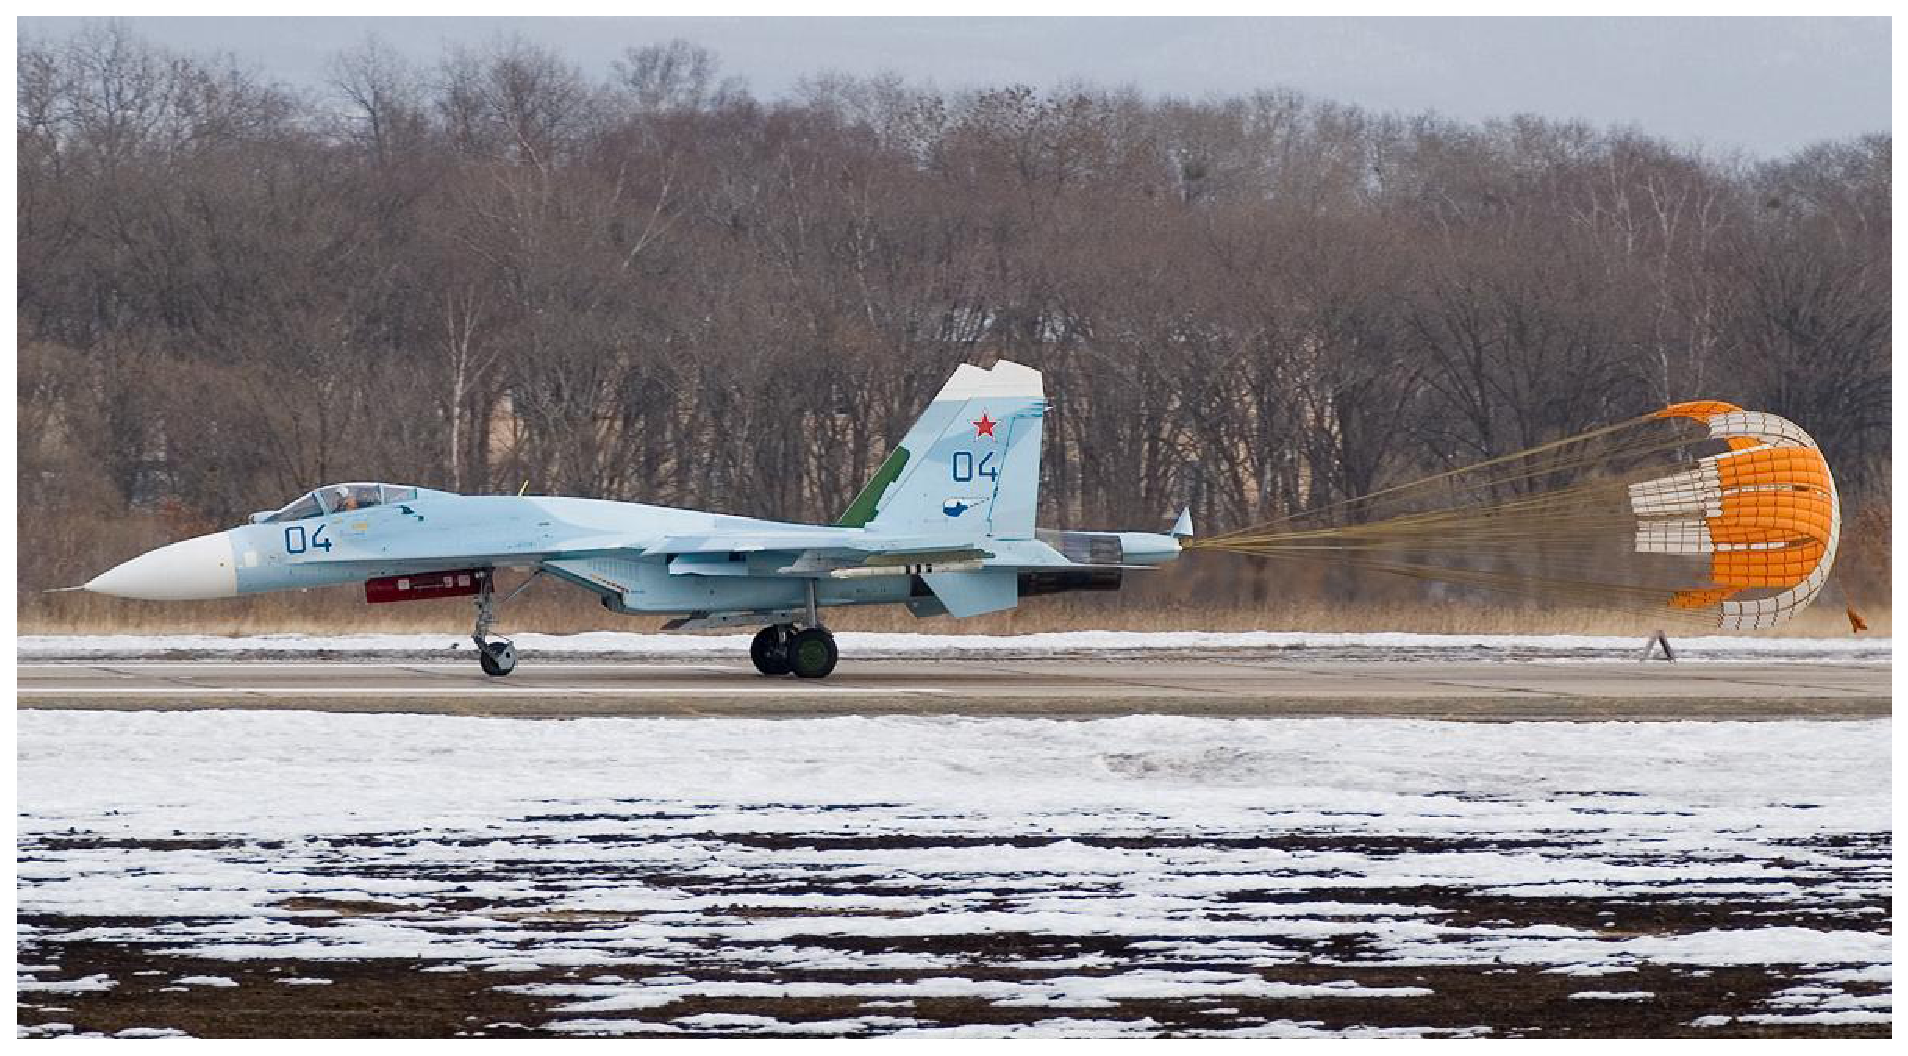
\includegraphics[keepaspectratio=true,width=0.6\linewidth]{midterm/dragchute.eps}
\caption{Drag chute}
\label{fig:e1}
\end{figure}
\begin{itemize}
\item[(a)] 감속하는 전투기의 속도에 대한 수학적모델을 세우고, 독립변수와 종속변수를 나타내시오. [5점]
\item[(b)] 감속하는 전투기의 속도 $80m/s$에서 $10m/s$에 도달하기 까지 걸리는 시간의 해석해(exact solution)를 구하시오. [10점]
\item[(c)] 문제(b)에서 동일하게 감속하는 시간동안 이동한 거리의 해석해(exact solution) 혹은 Euler법을 사용한 수치해(numerical solution)을 구하시오. (단, 수치해를 구할때 독립변수의 간격은 1로 하고, 각 단계에서의 절단오차 소숫점 4째자리의 과학적 표기법으로 나타내시오) [10점]
\end{itemize}

\begin{itemize}
\item[문제2] 다음 Figure\ref{fig:e2}는 등분포하중을 받는 캔틸레버보를 나타낸다. 탄성곡선의 방정식은 식(\ref{eq:e2})와 같다. 다음 문항에 답하여라.
\end{itemize}
\begin{figure}[!hbpt]
\centering
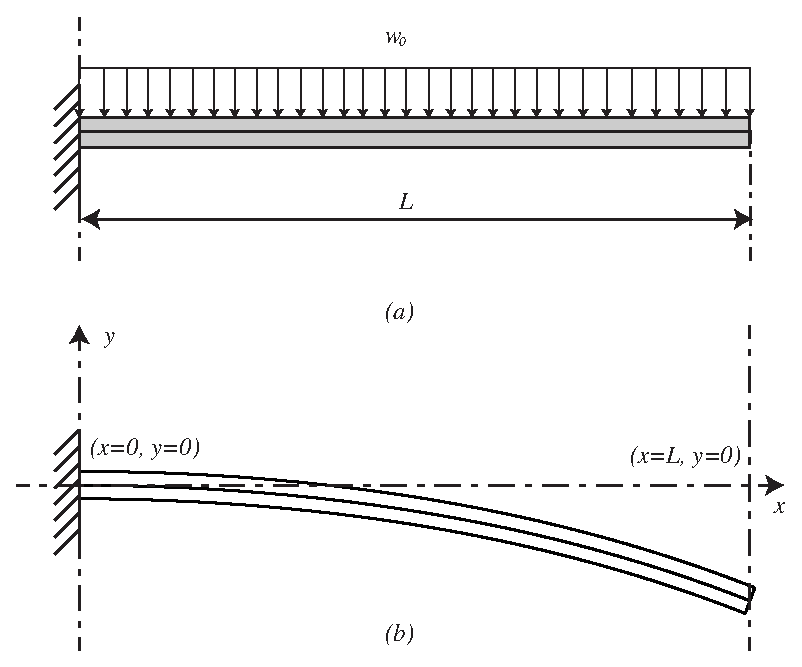
\includegraphics[keepaspectratio=true,width=0.6\linewidth]{midterm/2.eps}
\caption{Cantilever beam}
\label{fig:e2}
\end{figure}

\begin{equation}\label{eq:e2}
y=\frac{w_{0}}{24EI}\left(-x^4+4Lx^3-6L^2 x^2\right)
\end{equation}
\begin{itemize}
\item[(a)] 캔틸레버보의 $x=50cm$일 때를 기준점으로 하여 0차에서 3차까지의 Taylor급수전개를 사용하여 $x=100cm$지점의 처짐($y$)의 근사값을 구하고, 참백분율 상대오차 $\epsilon_{t}$를 구하라. (단, 매개변수는 $L=300cm$, $E=50,000kN/cm^2$, $I=30,000cm^4$, $w_{0}=2.5kN/cm$과 같다.) [10점]
\item[(b)] (a)의 매개변수에서 $L=300\pm5cm$ 그리고 $I=30,000\pm100cm^4$의 측정오차가 있었다. 1차 오차해석으로 $x=100cm$ 지점에서의 처짐각($dy/dx$)의 추정오차값을 구하여라. (단, 절단오차는 소수점 4째 자리의 과학적 표기법으로 표시한다.) [10점]
\item[(c)] 처짐($y$)이 $2cm$가 되는 지점을 이분법을 사용하여 근을 구하라, $x_{l}=200cm$, $x_{u}=250cm$을 초기구간으로 가정하고, 근사오차 $\epsilon_{a}$가 1\% 이하로 떨어질 때까지 반복하라. [10점] (단, 반복횟수만큼의 열을 가지는 테이블을 작성하고 함수값등의 절단오차는 소수점 4째 자리의 과학적 표기법으로 표시한다.)
\end{itemize}

\begin{itemize}
\item[문제3] 물체의 점성감쇠조화진동(harmonic vibration with viscoud damping)이 공진상태까지 도달할 때, 정적변위응답($u_{st}$)에 대한 동적변위응답($u(t)$)은 다음 식(\ref{eq:e3})과 같이 주어진다. $\xi$가 $0$에 가까울 때, $\omega_{D}=\omega_{n}$으로, $\xi/\sqrt{1-\xi^2}=0$으로 근사화된 식(\ref{eq:e4})이 된다. 다음 문항에 답하여라.
\end{itemize}
\begin{align}
u(t)&=u_{st}\frac{1}{2\xi}\left[e^{-\xi\omega_{n}t}\left(\cos\omega_{D}t+\frac{\xi}{\sqrt{1-\xi^2}}\sin\omega_{D}t\right)-\cos\omega_{n}t\right]\label{eq:e3}\\
&\cong u_{st}\frac{1}{2\xi}\left(e^{-\xi\omega_{n}t}-1\right)\cos\omega_{n}t\label{eq:e4}
\end{align}
여기서, $\xi$는 감쇠비, $\omega_{n}$은 고유진동수 그리고 $\omega_{D}$는 감쇠고유진동수 $\omega_{D}=\omega_{n}/\sqrt{1-\xi^2}$이다.
\begin{itemize}
\item[(a)] $\omega_{n}=1$이고, $\xi=0.05$일 때, 식(\ref{eq:e4})을 통해 최대변위증폭비 $\max\{u(t)\}/u_{st}$가 5에 도달하는 시간을 Newton-Raphson법을 통해 구하여라. 초기가정 $x_{0}=10$으로 세번 반복한다. [15점]
\item[(b)] (a)를 할선법(secant method)를 사용하여 구하여라. 초기가정 $x_{0}=10$, $x_{1}=11$으로 시작하고 세번 반복하라 [15점]
\item[(c)] (a)를 수정된 할선법(modified secant method)를 사용하여 구하여라. 초기가정 $x_{0}=10$, $\delta=0.01$로 시작하고 세번 반복하라 [15점]
\item[$\blacktriangleright$]유의사항 : 최대변위증폭비이기 때문에 $\max(\cos\omega_{n}t)=1$로 가정한 포락곡선함수(envelope function)를 사용하고, 증폭비는 절대값이기 때문에 포락곡선함수의 근의 존재유무에 유의하라.
\end{itemize}
\clearpage

\begin{algorithm}\label{alg:c5}
Choose lower $x_{l}$ and upper $x_{u}$ guesses for the root such that the function changes sign over the interval. This can be checked by ensuring that $f(x_{l})f(x_{u})<0$.
\begin{algorithmic}
\While{$f(x_{r})$ is not sufficiently small}
  \State $x_{r}=\frac{x_{l}+x_{u}}{2}$
  \If{$f(x_{l})f(x_{r})<0$}
    \State $x_{u}=x_{r}$
  \Else
    \State $x_{l}=x_{r}$
  \EndIf  
  \If{$\epsilon_{a}=\left|\frac{x_{new}-x_{old}}{x_{new}}\right|$ is sufficiently small}
    \State $x_{r}=x_{new}$
    \State \Return $x_{r}$
  \EndIf
\EndWhile
\end{algorithmic}
\caption{이분법(Bisection Method)}
\end{algorithm}

\begin{algorithm}\label{alg:c1}
Choose an initial guess $x_{0}$.
\begin{algorithmic}
\For{$i=0,1,2,\cdots$}
  \If{$f(x_{i})$ is sufficiently small}
    \State $x_{r}=x_{i}$
    \State \Return $x_{r}$
  \EndIf
  \State $x_{i+1}=x_{i}-\frac{f(x_{i})}{f'(x_{i})}$
  \If{$\left|x_{i+1}-x_{i}\right|$ is sufficiently small}
    \State $x_{r}=x_{i+1}$
    \State \Return $x_{r}$
  \EndIf
\EndFor
\end{algorithmic}
\caption{Newton-Raphson Method}
\end{algorithm}

\begin{algorithm}\label{alg:c2}
Choose an initial guess $x_{0}$ and $x_{1}$.
\begin{algorithmic}
\For{$i=0,1,2,\cdots$}
  \If{$f(x_{i})$ is sufficiently small}
    \State $x_{r}=x_{i}$
    \State \Return $x_{r}$
  \EndIf
  \State $x_{i+2}=x_{i+1}-\frac{f(x_{i+1})(x_{i}-x_{i+1})}{f(x_{i})-f(x_{i+1})}$
  \If{$\left|x_{i+2}-x_{i+1}\right|$ is sufficiently small}
    \State $x_{r}=x_{i+2}$
    \State \Return $x_{r}$
  \EndIf
\EndFor
\end{algorithmic}
\caption{Secant Method}
\end{algorithm}

\begin{algorithm}\label{alg:c3}
Choose an initial guess $x_{0}$ and $\delta$.
\begin{algorithmic}
\For{$i=0,1,2,\cdots$}
  \If{$f(x_{i})$ is sufficiently small}
    \State $x_{r}=x_{i}$
    \State \Return $x_{r}$
  \EndIf
  \State $x_{i+1}=x_{i}-\frac{\delta x_{i}f(x_{i})}{f(x_{i}+\delta x_{i})-f(x_{i})}$
  \If{$\left|x_{i+1}-x_{i}\right|$ is sufficiently small}
    \State $x_{r}=x_{i+1}$
    \State \Return $x_{r}$
  \EndIf
\EndFor
\end{algorithmic}
\caption{Modified Secant Method}
\end{algorithm}

\end{document}
